% Options for packages loaded elsewhere
% Options for packages loaded elsewhere
\PassOptionsToPackage{unicode}{hyperref}
\PassOptionsToPackage{hyphens}{url}
%
\documentclass[
  10pt,
  ignorenonframetext,
  aspectratio=169,
  russian,
]{beamer}
\newif\ifbibliography
\usepackage{pgfpages}
\setbeamertemplate{caption}[numbered]
\setbeamertemplate{caption label separator}{: }
\setbeamercolor{caption name}{fg=normal text.fg}
\beamertemplatenavigationsymbolshorizontal
% remove section numbering
\setbeamertemplate{part page}{
  \centering
  \begin{beamercolorbox}[sep=16pt,center]{part title}
    \usebeamerfont{part title}\insertpart\par
  \end{beamercolorbox}
}
\setbeamertemplate{section page}{
  \centering
  \begin{beamercolorbox}[sep=12pt,center]{section title}
    \usebeamerfont{section title}\insertsection\par
  \end{beamercolorbox}
}
\setbeamertemplate{subsection page}{
  \centering
  \begin{beamercolorbox}[sep=8pt,center]{subsection title}
    \usebeamerfont{subsection title}\insertsubsection\par
  \end{beamercolorbox}
}
% Prevent slide breaks in the middle of a paragraph
\widowpenalties 1 10000
\raggedbottom
\AtBeginPart{
  \frame{\partpage}
}
\AtBeginSection{
  \ifbibliography
  \else
    \frame{\sectionpage}
  \fi
}
\AtBeginSubsection{
  \frame{\subsectionpage}
}
\usepackage{iftex}
\ifPDFTeX
  \usepackage[T1]{fontenc}
  \usepackage[utf8]{inputenc}
  \usepackage{textcomp} % provide euro and other symbols
\else % if luatex or xetex
  \usepackage{unicode-math} % this also loads fontspec
  \defaultfontfeatures{Scale=MatchLowercase}
  \defaultfontfeatures[\rmfamily]{Ligatures=TeX,Scale=1}
\fi
\usepackage{lmodern}

\usetheme[]{metropolis}
\usefonttheme{serif} % use mainfont rather than sansfont for slide text
\ifPDFTeX\else
  % xetex/luatex font selection
  \setmainfont[]{DejaVu Sans}
  \setsansfont[]{DejaVu Sans}
  \setmonofont[]{DejaVu Sans Mono}
\fi
% Use upquote if available, for straight quotes in verbatim environments
\IfFileExists{upquote.sty}{\usepackage{upquote}}{}
\IfFileExists{microtype.sty}{% use microtype if available
  \usepackage[]{microtype}
  \UseMicrotypeSet[protrusion]{basicmath} % disable protrusion for tt fonts
}{}


\usepackage{longtable,booktabs,array}
\newcounter{none} % for unnumbered tables
\usepackage{calc} % for calculating minipage widths
\usepackage{caption}
% Make caption package work with longtable
\makeatletter
\def\fnum@table{\tablename~\thetable}
\makeatother
\usepackage{graphicx}
\makeatletter
\newsavebox\pandoc@box
\newcommand*\pandocbounded[1]{% scales image to fit in text height/width
  \sbox\pandoc@box{#1}%
  \Gscale@div\@tempa{\textheight}{\dimexpr\ht\pandoc@box+\dp\pandoc@box\relax}%
  \Gscale@div\@tempb{\linewidth}{\wd\pandoc@box}%
  \ifdim\@tempb\p@<\@tempa\p@\let\@tempa\@tempb\fi% select the smaller of both
  \ifdim\@tempa\p@<\p@\scalebox{\@tempa}{\usebox\pandoc@box}%
  \else\usebox{\pandoc@box}%
  \fi%
}
% Set default figure placement to htbp
\def\fps@figure{htbp}
\makeatother



\ifLuaTeX
\usepackage[bidi=basic,shorthands=off,provide=*]{babel}
\else
\usepackage[bidi=default,shorthands=off,provide=*]{babel}
\fi
\ifPDFTeX
\else
\babelfont{rm}[]{DejaVu Sans}
\fi
\ifLuaTeX
  \usepackage{selnolig} % disable illegal ligatures
\fi


\setlength{\emergencystretch}{3em} % prevent overfull lines

\providecommand{\tightlist}{%
  \setlength{\itemsep}{0pt}\setlength{\parskip}{0pt}}



 

\usepackage[]{csquotes}

%%% Load theme
\IfFileExists{beamerthemegotham.sty}{
  %%%% Full TeXlive
  \usetheme{gotham}
  \gothamset{
    numbering=totalframenumber,
    parttocframe default=off,
    sectiontocframe default=off,
    subsectiontocframe default=off,
    tocframe template=gotham bullet,
    % progressbar position=frametitle,
    progressbar position=foot,
  }
  \renewcommand{\gothamInstituteLogoSquare}[1][4ex]{%
    
\includegraphics[height=##1]{_resources/image/logo_rudn-inverted.png}
  }
  % \renewcommand{\gothamtitlepagelogo}[1][4ex]{%
  %   
\includegraphics[height=##1]{_resources/image/logo_rudn.png}
  % }
}{%
  %%%% TinyTeX
  \usepackage{libertine}
  %%%% https://deic.uab.cat/~iblanes/beamer_gallery/
  \usetheme{Madrid}
}
\metroset{progressbar=frametitle,numbering=fraction}
\setbeamersize{text margin left=8mm,text margin right=8mm}
\makeatletter
\@ifpackageloaded{caption}{}{\usepackage{caption}}
\AtBeginDocument{%
\ifdefined\contentsname
  \renewcommand*\contentsname{Содержание}
\else
  \newcommand\contentsname{Содержание}
\fi
\ifdefined\listfigurename
  \renewcommand*\listfigurename{Список иллюстраций}
\else
  \newcommand\listfigurename{Список иллюстраций}
\fi
\ifdefined\listtablename
  \renewcommand*\listtablename{Список таблиц}
\else
  \newcommand\listtablename{Список таблиц}
\fi
\ifdefined\figurename
  \renewcommand*\figurename{Рисунок}
\else
  \newcommand\figurename{Рисунок}
\fi
\ifdefined\tablename
  \renewcommand*\tablename{Таблица}
\else
  \newcommand\tablename{Таблица}
\fi
}
\@ifpackageloaded{float}{}{\usepackage{float}}
\floatstyle{ruled}
\@ifundefined{c@chapter}{\newfloat{codelisting}{h}{lop}}{\newfloat{codelisting}{h}{lop}[chapter]}
\floatname{codelisting}{Список}
\newcommand*\listoflistings{\listof{codelisting}{Листинги}}
\makeatother
\makeatletter
\makeatother
\makeatletter
\@ifpackageloaded{caption}{}{\usepackage{caption}}
\@ifpackageloaded{subcaption}{}{\usepackage{subcaption}}
\makeatother

\usepackage{bookmark}
\IfFileExists{xurl.sty}{\usepackage{xurl}}{} % add URL line breaks if available
\urlstyle{same}
% fallback for those not using the hyperref driver hyperxmp:
\makeatletter
\@ifundefined{xmpquote}{\newcommand{\xmpquote}[1]{#1}}{}
\makeatother
\hypersetup{
  pdftitle={Лабораторная работа № 2},
  pdfauthor={Нечаева Кира Андреевна},
  pdflang={ru-RU},
  hidelinks,
  pdfcreator={LaTeX via pandoc}}


\title{\texorpdfstring{Лабораторная работа №
2}{Лабораторная работа № 2}}
\subtitle{\texorpdfstring{Модели SIR и
Лотки--Вольтерры}{Модели SIR и Лотки--Вольтерры}}
\author{Нечаева Кира Андреевна}
\date{}
\institute{НКНбд-01-23}

\begin{document}
\frame{\titlepage}


\begin{frame}{Цель работы}
\protect\phantomsection\label{ux446ux435ux43bux44c-ux440ux430ux431ux43eux442ux44b}
\textbf{Цель:} реализовать и исследовать две системы имитационного
моделирования средствами Julia.

В работе:

\begin{itemize}
\tightlist
\item
  реализована эпидемиологическая модель SIR;
\item
  реализована модель Лотки--Вольтерры;
\item
  проведены параметрические эксперименты;
\item
  построены графики результатов;
\item
  код преобразован в Julia, Quarto и Jupyter Notebook.
\end{itemize}
\end{frame}

\begin{frame}[fragile]{Рабочее окружение}
\protect\phantomsection\label{ux440ux430ux431ux43eux447ux435ux435-ux43eux43aux440ux443ux436ux435ux43dux438ux435}
\begin{columns}[c]
\begin{column}{0.38\linewidth}
Для работы создан отдельный проект DrWatson.

Использованы:

\begin{itemize}
\tightlist
\item
  \texttt{DifferentialEquations};
\item
  \texttt{DataFrames};
\item
  \texttt{Plots};
\item
  \texttt{StatsPlots};
\item
  \texttt{BenchmarkTools};
\item
  \texttt{FFTW};
\item
  \texttt{Literate};
\item
  \texttt{IJulia}.
\end{itemize}
\end{column}

\begin{column}{0.62\linewidth}
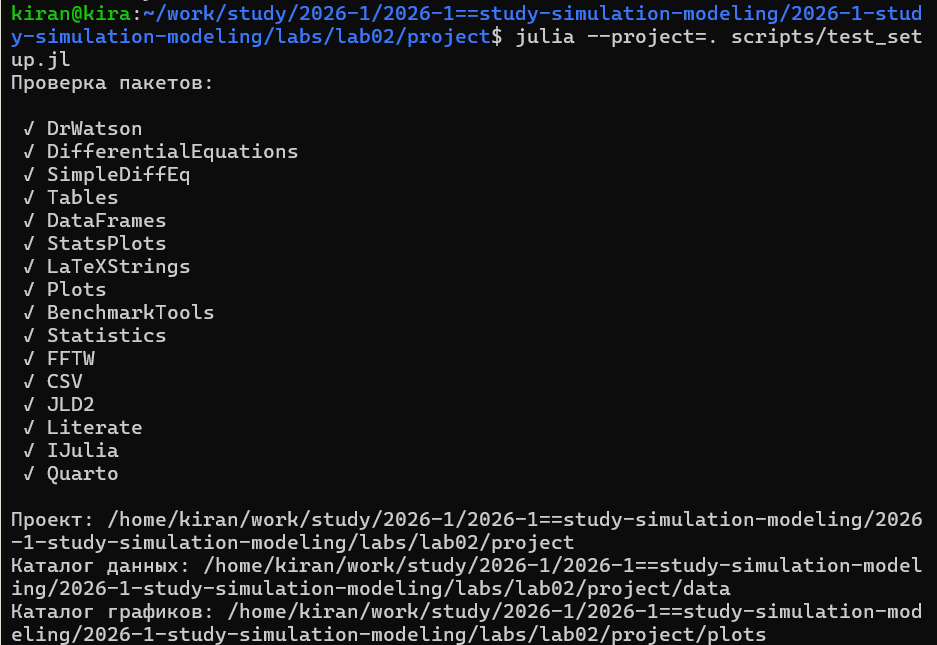
\includegraphics[width=1\linewidth,height=\textheight,keepaspectratio]{image/2.png}
\end{column}
\end{columns}
\end{frame}

\begin{frame}{Модель SIR}
\protect\phantomsection\label{ux43cux43eux434ux435ux43bux44c-sir}
\begin{columns}[c]
\begin{column}{0.35\linewidth}
Популяция разделяется на три группы:

\begin{itemize}
\tightlist
\item
  \(S\) --- восприимчивые;
\item
  \(I\) --- инфицированные;
\item
  \(R\) --- выздоровевшие.
\end{itemize}

Базовые параметры:

\[
\beta=0.05,\qquad
c=10,\qquad
\gamma=0.25.
\]

В базовом эксперименте

\[
R_0=\frac{c\beta}{\gamma}=2.
\]
\end{column}

\begin{column}{0.65\linewidth}
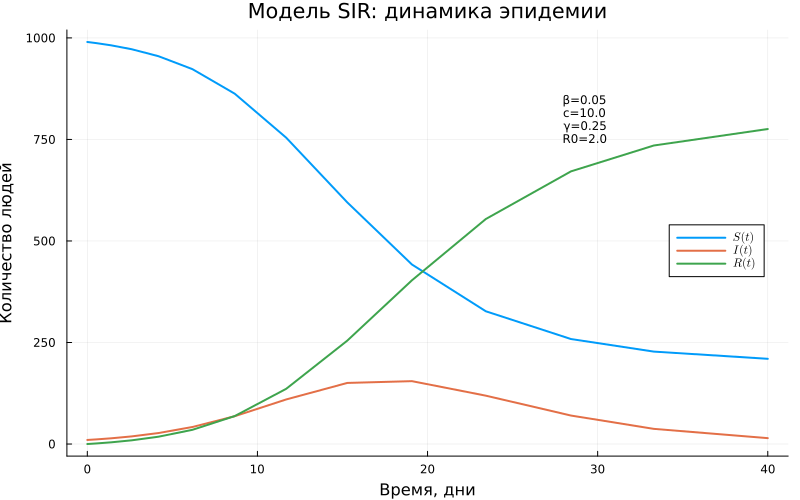
\includegraphics[width=1\linewidth,height=\textheight,keepaspectratio]{image/plots/sir_main.png}
\end{column}
\end{columns}
\end{frame}

\begin{frame}{Динамика эпидемии}
\protect\phantomsection\label{ux434ux438ux43dux430ux43cux438ux43aux430-ux44dux43fux438ux434ux435ux43cux438ux438}
\begin{columns}[c]
\begin{column}{0.32\linewidth}
В начале число инфицированных увеличивается.

По мере сокращения числа восприимчивых эффективное репродуктивное число
уменьшается.

Когда \(R_e<1\), распространение инфекции начинает затухать.
\end{column}

\begin{column}{0.68\linewidth}
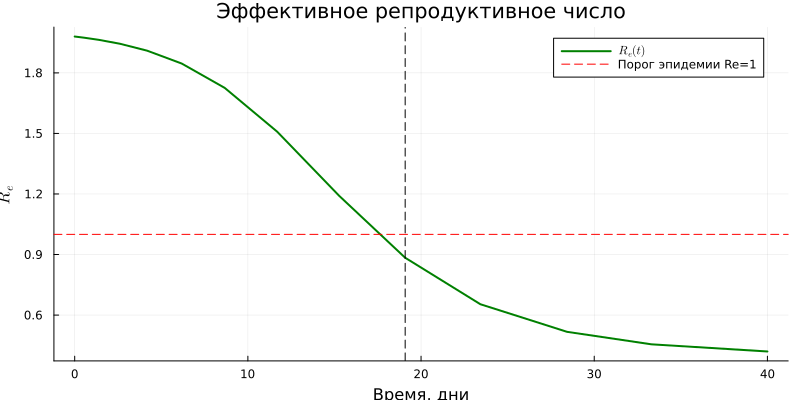
\includegraphics[width=1\linewidth,height=\textheight,keepaspectratio]{image/plots/sir_effective_R.png}
\end{column}
\end{columns}
\end{frame}

\begin{frame}{Параметрическое исследование SIR}
\protect\phantomsection\label{ux43fux430ux440ux430ux43cux435ux442ux440ux438ux447ux435ux441ux43aux43eux435-ux438ux441ux441ux43bux435ux434ux43eux432ux430ux43dux438ux435-sir}
\begin{columns}[c]
\begin{column}{0.3\linewidth}
В серии экспериментов изменялось среднее число контактов \(c\).

Остальные параметры сохранялись постоянными.

Так можно отдельно оценить влияние интенсивности контактов на развитие
эпидемии.
\end{column}

\begin{column}{0.7\linewidth}
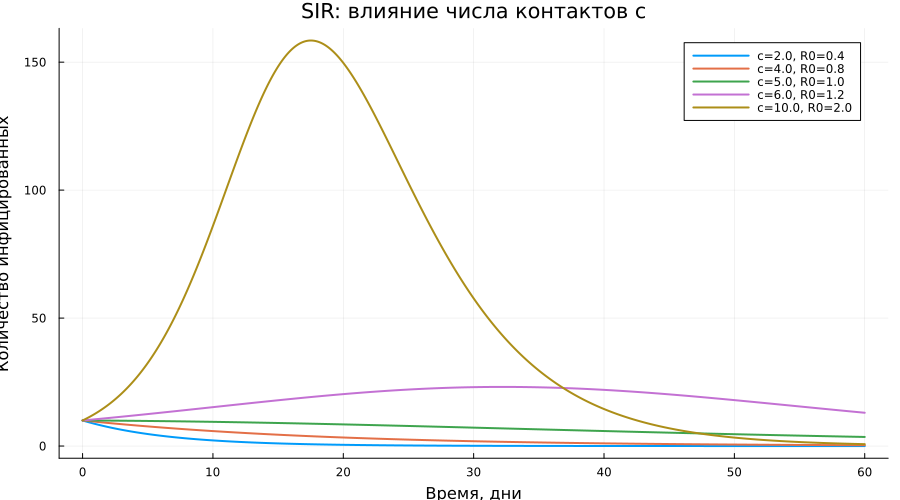
\includegraphics[width=1\linewidth,height=\textheight,keepaspectratio]{image/plots/sir_contact_scan.png}
\end{column}
\end{columns}
\end{frame}

\begin{frame}{Воспроизводимость SIR}
\protect\phantomsection\label{ux432ux43eux441ux43fux440ux43eux438ux437ux432ux43eux434ux438ux43cux43eux441ux442ux44c-sir}
\begin{columns}[c]
\begin{column}{0.36\linewidth}
Один литературный исходник автоматически преобразован в:

\begin{itemize}
\tightlist
\item
  исполняемый Julia-код;
\item
  Quarto-документ;
\item
  Jupyter Notebook.
\end{itemize}

Обе версии SIR были выполнены в Jupyter.
\end{column}

\begin{column}{0.64\linewidth}
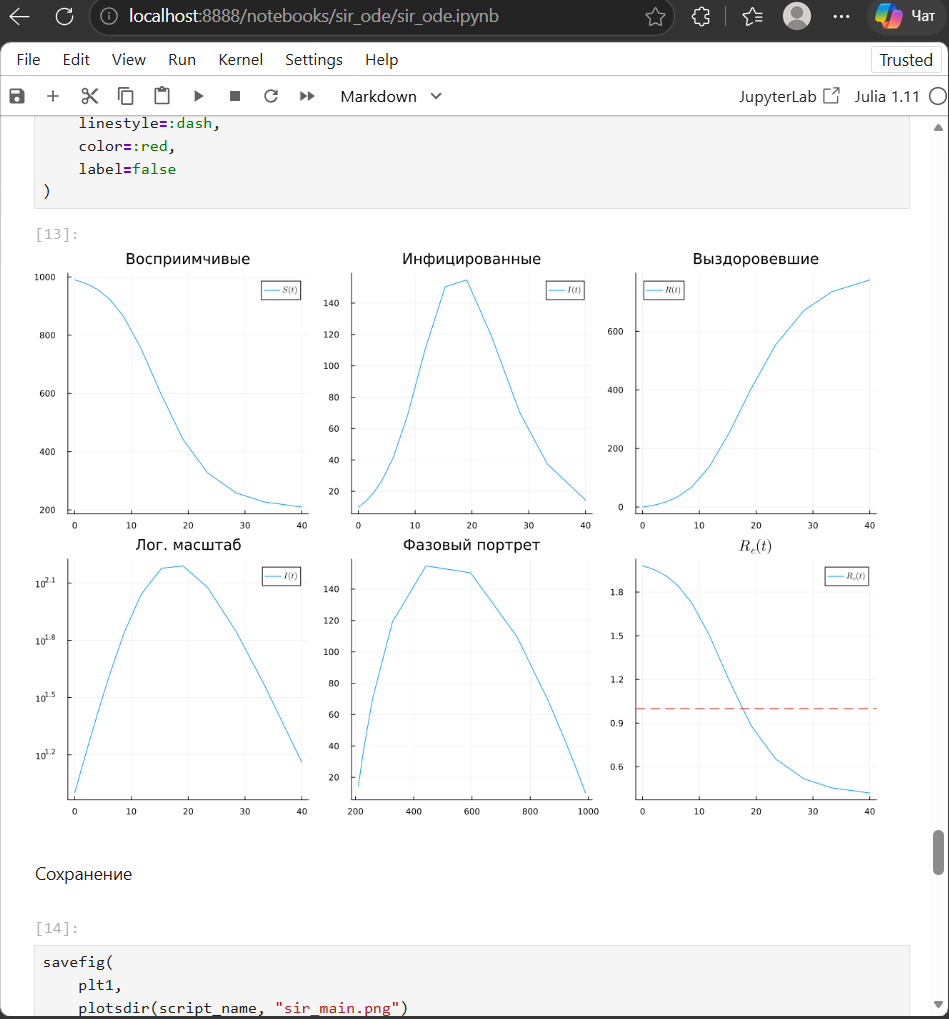
\includegraphics[width=1\linewidth,height=\textheight,keepaspectratio]{image/10.png}
\end{column}
\end{columns}
\end{frame}

\begin{frame}{Модель Лотки--Вольтерры}
\protect\phantomsection\label{ux43cux43eux434ux435ux43bux44c-ux43bux43eux442ux43aux438ux432ux43eux43bux44cux442ux435ux440ux440ux44b}
\begin{columns}[c]
\begin{column}{0.34\linewidth}
Модель описывает взаимодействие двух популяций:

\begin{itemize}
\tightlist
\item
  \(x\) --- жертвы;
\item
  \(y\) --- хищники.
\end{itemize}

Параметры:

\[
\alpha=0.1,\quad
\beta=0.02,
\]

\[
\delta=0.01,\quad
\gamma=0.3.
\]

Начальное состояние:

\[
x_0=40,\qquad y_0=9.
\]
\end{column}

\begin{column}{0.66\linewidth}
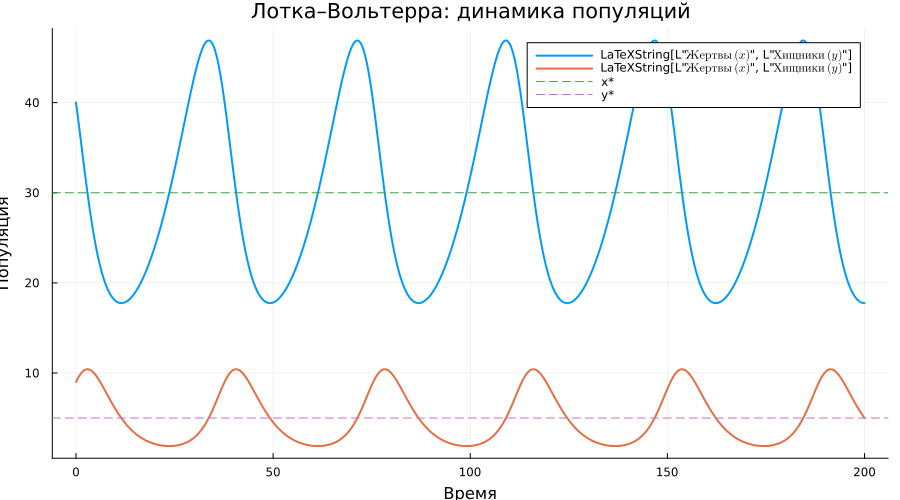
\includegraphics[width=1\linewidth,height=\textheight,keepaspectratio]{image/plots/lv_dynamics.png}
\end{column}
\end{columns}
\end{frame}

\begin{frame}{Циклическая динамика}
\protect\phantomsection\label{ux446ux438ux43aux43bux438ux447ux435ux441ux43aux430ux44f-ux434ux438ux43dux430ux43cux438ux43aux430}
\begin{columns}[c]
\begin{column}{0.31\linewidth}
Сначала увеличивается число жертв.

Рост числа жертв создаёт больше ресурсов для хищников, поэтому их
максимум наступает позже.

После роста хищников численность жертв снова уменьшается, и цикл
повторяется.
\end{column}

\begin{column}{0.69\linewidth}
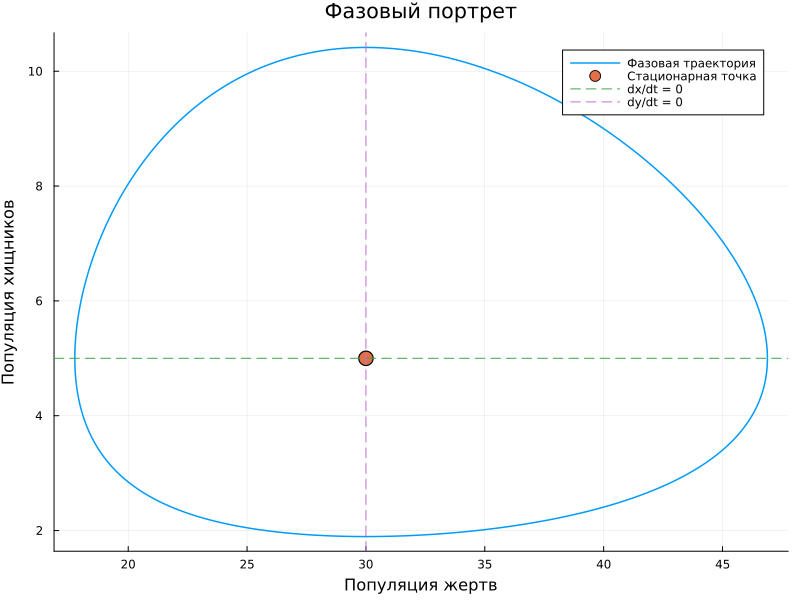
\includegraphics[width=0.95\linewidth,height=\textheight,keepaspectratio]{image/plots/lv_phase_portrait.png}
\end{column}
\end{columns}
\end{frame}

\begin{frame}{Параметрическое исследование}
\protect\phantomsection\label{ux43fux430ux440ux430ux43cux435ux442ux440ux438ux447ux435ux441ux43aux43eux435-ux438ux441ux441ux43bux435ux434ux43eux432ux430ux43dux438ux435}
\begin{columns}[c]
\begin{column}{0.3\linewidth}
Отдельно исследовались:

\textbf{\(\alpha\)} --- скорость естественного роста жертв;

\textbf{\(\gamma\)} --- скорость естественной смертности хищников.

При изменении параметров меняются амплитуда и характер колебаний
системы.
\end{column}

\begin{column}{0.7\linewidth}
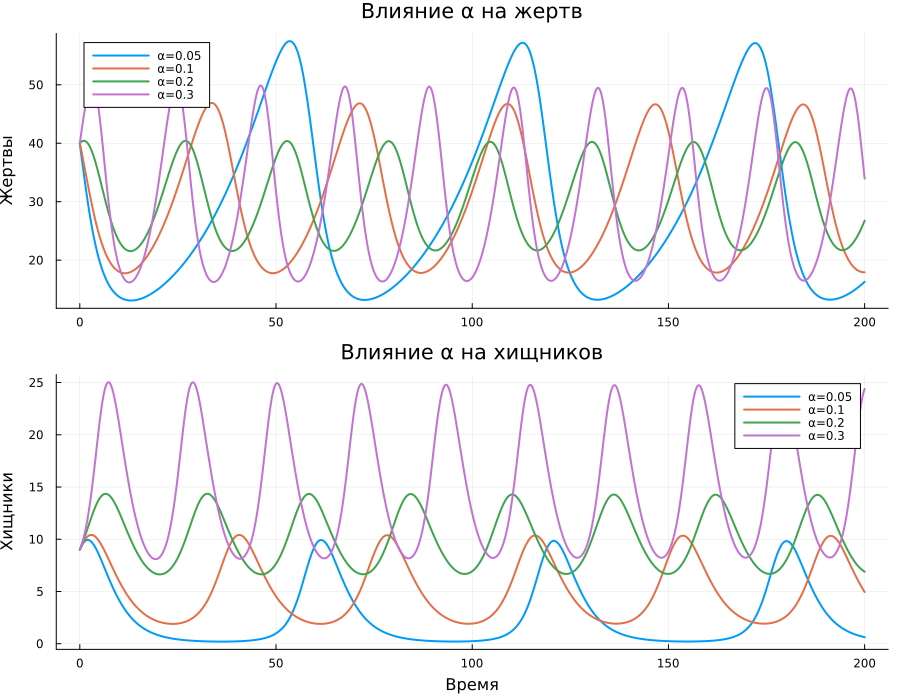
\includegraphics[width=1\linewidth,height=\textheight,keepaspectratio]{image/plots/lv_alpha_scan.png}
\end{column}
\end{columns}
\end{frame}

\begin{frame}{Влияние смертности хищников}
\protect\phantomsection\label{ux432ux43bux438ux44fux43dux438ux435-ux441ux43cux435ux440ux442ux43dux43eux441ux442ux438-ux445ux438ux449ux43dux438ux43aux43eux432}
\begin{columns}[c]
\begin{column}{0.3\linewidth}
При изменении \(\gamma\) изменяется скорость уменьшения популяции
хищников.

Это влияет не только на численность хищников, но и на последующую
динамику жертв.
\end{column}

\begin{column}{0.7\linewidth}
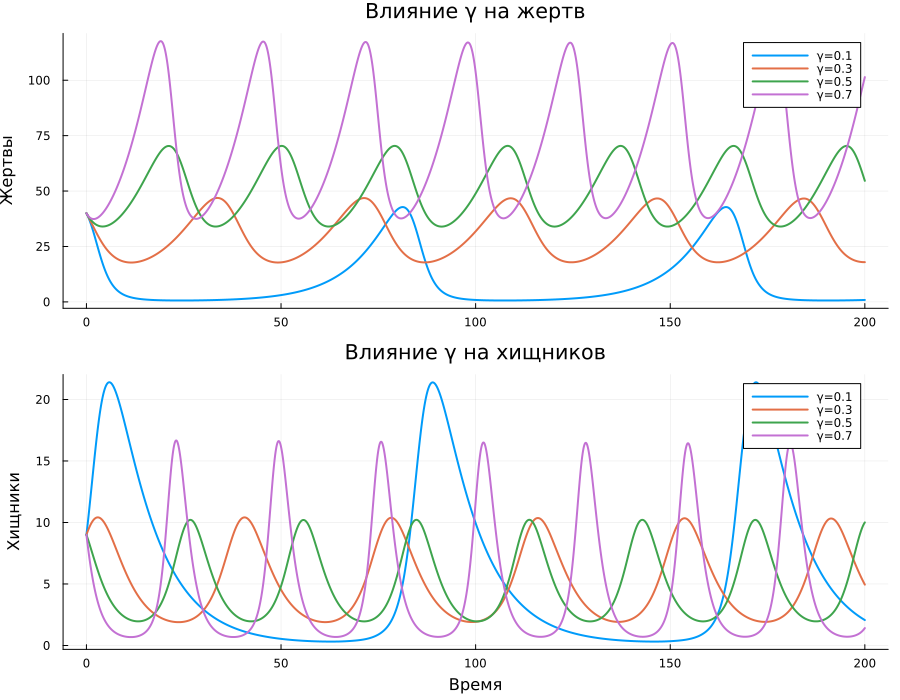
\includegraphics[width=1\linewidth,height=\textheight,keepaspectratio]{image/plots/lv_gamma_scan.png}
\end{column}
\end{columns}
\end{frame}

\begin{frame}{Литературное программирование}
\protect\phantomsection\label{ux43bux438ux442ux435ux440ux430ux442ux443ux440ux43dux43eux435-ux43fux440ux43eux433ux440ux430ux43cux43cux438ux440ux43eux432ux430ux43dux438ux435}
\begin{columns}[c]
\begin{column}{0.38\linewidth}
Для обеих моделей и их параметрических версий сформированы:

\begin{itemize}
\tightlist
\item
  чистые Julia-скрипты;
\item
  Quarto-документация;
\item
  Jupyter Notebook;
\item
  данные;
\item
  графики.
\end{itemize}
\end{column}

\begin{column}{0.62\linewidth}
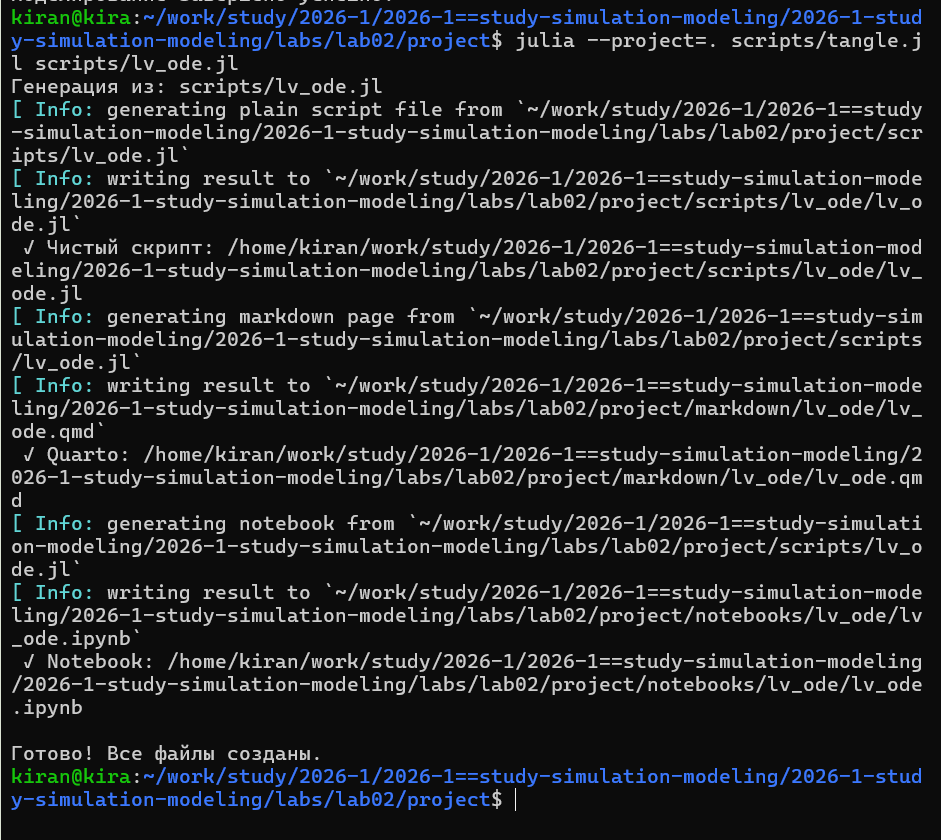
\includegraphics[width=1\linewidth,height=\textheight,keepaspectratio]{image/16.png}
\end{column}
\end{columns}
\end{frame}

\begin{frame}{Итоговая структура}
\protect\phantomsection\label{ux438ux442ux43eux433ux43eux432ux430ux44f-ux441ux442ux440ux443ux43aux442ux443ux440ux430}
\begin{columns}[c]
\begin{column}{0.37\linewidth}
В результате получен воспроизводимый проект, в котором исходный код,
результаты вычислений, графики и документация связаны между собой.

Все результаты сохранены в системе контроля версий.
\end{column}

\begin{column}{0.63\linewidth}
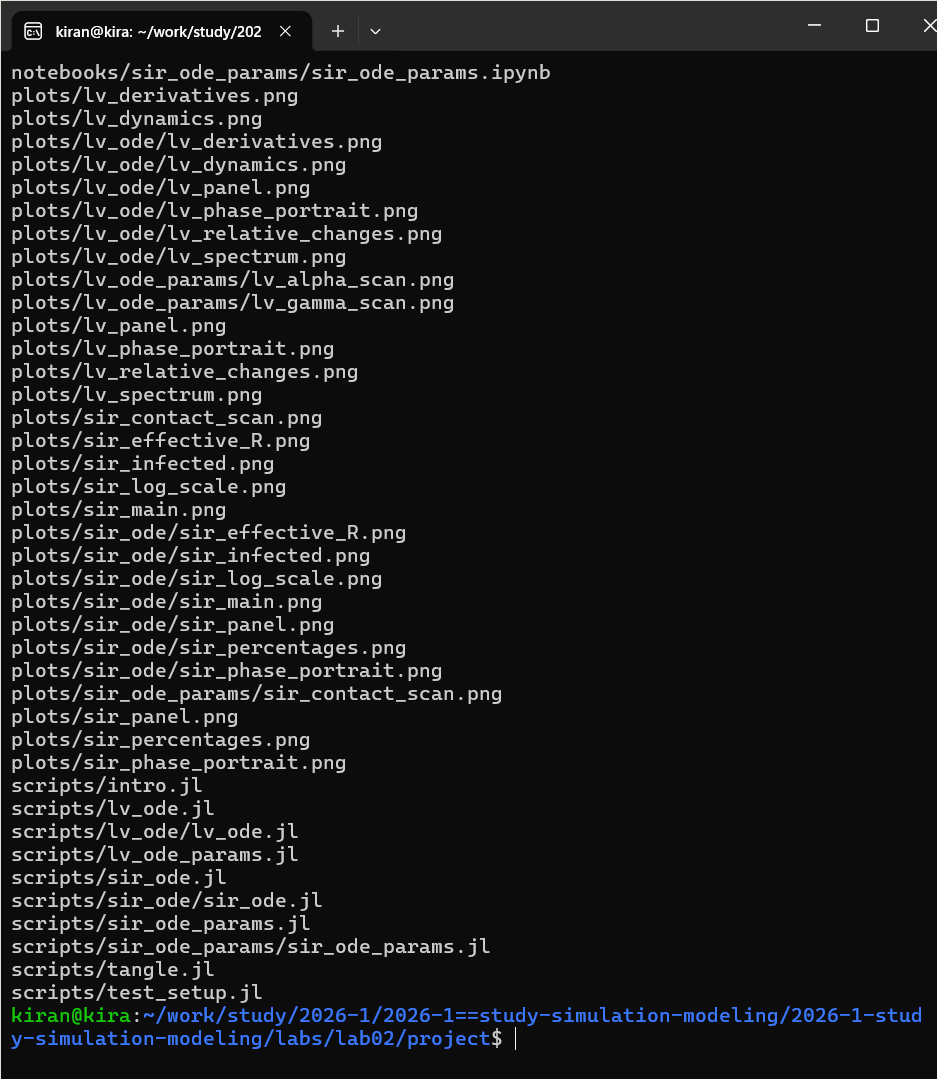
\includegraphics[width=1\linewidth,height=\textheight,keepaspectratio]{image/21.png}
\end{column}
\end{columns}
\end{frame}

\begin{frame}{Выводы}
\protect\phantomsection\label{ux432ux44bux432ux43eux434ux44b}
В лабораторной работе были реализованы две модели.

\begin{itemize}
\tightlist
\item
  SIR показывает переход населения между группами восприимчивых,
  инфицированных и выздоровевших.
\item
  Уменьшение числа контактов снижает скорость распространения инфекции.
\item
  Модель Лотки--Вольтерры демонстрирует циклическое взаимодействие
  хищников и жертв.
\item
  Изменение параметров \(\alpha\) и \(\gamma\) заметно меняет динамику
  системы.
\item
  Все вычисления оформлены как воспроизводимый Julia-проект.
\end{itemize}

\textbf{Исходный код, результаты и документация формируются программно.}
\end{frame}




\end{document}
